\documentclass[10pt,a4paper]{article}
\usepackage{amsmath,amssymb,graphicx,booktabs,geometry,hyperref,microtype}
\geometry{margin=0.85in}
\setlength{\emergencystretch}{2em}
\hypersetup{colorlinks=true,urlcolor=blue,linkcolor=black}
\title{\textbf{When Training Fit Is Not Reasoning:\\Auditing ARC Search, Metrics, and Compute Budgets}}
\author{Team \texttt{krishnak} --- ARC Prize 2026 Paper Track}
\date{6 November 2026}
\begin{document}
\maketitle
\begin{abstract}
We report an artifact-backed audit of two ARC-AGI-2 systems: a symbolic/learned candidate-search system whose counted entry scored 0.00, and a reproduction of a public test-time-adapted Qwen3-4B pipeline whose late, unranked submission received 30.56. The contribution is a diagnostic account, not a new competitive model. First, the search implementation labels a task \texttt{solved} when it finds a training-consistent candidate: 20/120 such successes on public evaluation coexist with 0/120 graded test successes. Second, we identify two concrete canonical-key defects: colour normalisation before rotation fails dihedral invariance, and shape-free byte keys collide on non-equivalent rectangles. A corrected key passes 34,992 exhaustive transformation checks on all three-colour $2\times3$ grids. Third, twelve measured task latencies support a conditional scheduling experiment: 5,000 empirical-resampling runs complete a median 226/240 tasks within a 710-minute, four-worker budget; assumed 25\% and 50\% latency increases reduce that to 180 and 150. These are simulations, not hidden-set measurements or confidence bounds. We separate training fit, prediction availability, scored accuracy, and submission eligibility, and release an executable audit with source hashes. The lessons are actionable: preserve symmetry witnesses, grade unseen outputs, record coverage at the scoring-unit level, and leave queue slack before submitting.
\end{abstract}

\section{Scope and contribution}
ARC-AGI-2 evaluates generalisation from a few grid demonstrations rather than ordinary training fit \cite{arcagi2}. A useful solver must not only propose a rule but select correct unseen outputs and finish a valid submission. Our project exposed failures at all three interfaces.

\textbf{System A} generates candidates from a domain-specific primitive language, depth-2 composition, bidirectional search, and learned families (cell-tree, object-tree, patch lookup and MLP). \textbf{System B} reproduces \texttt{koushikrudra/failed-in-aimo}, version 1, using the public ARC-fine-tuned Qwen3-4B weights \cite{source,model}. We attribute the model, adaptation and decoding recipe to that notebook and its upstream dependencies; we claim no model or test-time-training novelty.

The contribution is threefold: (i) an implementation-level metric audit showing why candidate discovery was mistaken for solving, (ii) explicit counterexamples and a checked repair for canonicalisation, and (iii) a transparent, conditional scheduling analysis replacing unsupported hidden-coverage claims. We distinguish this new audit from historical runs: the search corrections were \emph{not} used in the closed main-track submission and have no demonstrated accuracy benefit yet.

\section{Candidate discovery is not test accuracy}
\subsection{What the implementation actually records}
In \texttt{search.py}, the return field is \texttt{solved=bool(hypotheses)}; in \texttt{solver\_v2.py}, it is \texttt{solved=bool(candidates)}. Candidate acceptance checks demonstration consistency. Neither assignment compares unseen test predictions with labels. Thus the field named \texttt{solve\_rate} is a \emph{candidate-discovery rate}, not a test solve rate.

We audited the two artifacts used by the earlier writeup (Table~\ref{tab:metrics}). The evaluation artifact is from the earlier cascade and the training artifact from the v2 solver: these are separate runs, not a matched generalisation experiment. The external grading counters are the accuracy measurements. Calling the 20 evaluation candidates ``20 solved grids'' would be incorrect.

\begin{table}[ht]
\centering
\caption{Historical artifacts, with corrected metric interpretation. Pass@1/2 here means exact task success under the local grader, using one/two submitted attempts.}
\label{tab:metrics}
\begin{tabular}{lrrrr}
\toprule
Artifact/split & Tasks & Candidate found & Graded pass@1 & Graded pass@2\\
\midrule
\texttt{training\_v2} & 150 & 41 (27.3\%) & 13 (8.7\%) & 13 (8.7\%)\\
\texttt{evaluation} & 120 & 20 (16.7\%) & 0 (0\%) & 0 (0\%)\\
\bottomrule
\end{tabular}
\end{table}

The candidate search therefore exhibits a \emph{fit-to-test gap}, not evidence of 16.7\% evaluation accuracy. The result does not alone identify the causal contribution of ranker overfitting, inadequate primitives, or search pruning. Distinguishing those requires an oracle candidate-accuracy experiment on held-out tasks.

\subsection{Reinterpreting the historical ablation}
The 60-task training ablation reports 25 candidate discoveries with the full cascade, 24 without depth-2, and 3 with symbolic families alone (8-second task budget). Removing learned families reduces candidate discovery by 22/60, or 36.7 percentage points. This supports a narrow conclusion: learned families drive most demonstration-consistent candidates in that run. It does \emph{not} establish that they improve unseen accuracy by 36.7 points. The 30-task evaluation ablation found four candidates; that is likewise not four demonstrated test solves.

\section{Canonicalisation: counterexamples and repair}
\subsection{Correct mathematical target}
Let $\mathcal G$ contain rectangular grids up to $30\times30$ with colours in $\{0,\ldots,9\}$. Dihedral actions rotate or reflect a grid (possibly swapping dimensions); colour permutations relabel its palette. Let $\operatorname{canon}$ replace each colour by its index of first appearance in row-major order. A dimension-preserving orbit key is
\begin{equation}
K(g)=\min_{r\in D_4}\bigl(h(rg),w(rg),\operatorname{bytes}(\operatorname{canon}(rg))\bigr).
\label{eq:key}
\end{equation}
Colour normalisation occurs \emph{inside} the minimisation, after each spatial transform.

\textbf{Proposition.} $K(r_0\pi g)=K(g)$ for every $r_0\in D_4$ and bijective colour permutation $\pi$. Moreover, equal keys imply orbit equivalence.

\textbf{Proof.} Colour renaming preserves the first-occurrence equality pattern, so $\operatorname{canon}(\pi x)=\operatorname{canon}(x)$. Spatial actions commute with pointwise colour renaming, and right multiplication by $r_0$ permutes $D_4$, leaving the minimum unchanged. If keys agree, their dimensions and canonical byte strings agree for some orientations. Matching first-occurrence classes induces a bijection between the used colours; combined with those orientations it maps one grid to the other. Unused palette colours can extend the bijection. $\square$

\subsection{Two verified implementation defects}
The actual \texttt{canonical\_key} first computes $\operatorname{canon}(g)$ and then minimises the bytes of its eight spatial variants. It does not implement Equation~\ref{eq:key}.

\textbf{Defect 1: order of operations.} The following two grids are related by a 180-degree rotation but the existing function returns different keys:
\[
g=\begin{pmatrix}0&0&0\\0&0&1\end{pmatrix},\qquad
r_{180}g=\begin{pmatrix}1&0&0\\0&0&0\end{pmatrix}.
\]
The transformed grid encounters colour 1 first, reversing the canonical labels before the spatial minimum. This produces a \emph{missed equivalence}, not evidence that the grids differ semantically.

\textbf{Defect 2: missing dimensions.} All-zero $1\times6$ and $2\times3$ grids both produce six zero bytes. They are not related by a dihedral transform or colour bijection. This is a \emph{false equivalence}. A caller would need a separate dimension guard to exclude it; the audited key itself has none.

The attached \texttt{corrected\_key} follows Equation~\ref{eq:key}. Enumerating all $3^6=729$ grids of shape $2\times3$, all eight spatial actions, and all $3!=6$ colour permutations gives $729\cdot8\cdot6=34{,}992$ successful invariance assertions. Separate assertions verify the original defects and that the corrected key distinguishes the shape collision. Exhaustive checks on this small domain support the implementation, while the proposition supplies the general argument.

\subsection{A key is not a compositional proof}
Even a correct orbit key cannot justify arbitrary search deduplication. A quotient search must either keep group-action witnesses and conjugate downstream operators or restrict transitions to compatible equivariant operators. Primitives that refer to absolute orientation or particular colours can distinguish two orbit-equivalent intermediates. Discarding one representative without its witness can therefore remove a valid continuation.

There is also a direction issue in bidirectional search. If forward operator $\alpha$ and backward operator $\beta$ satisfy
$\alpha(s)=\beta(d)$, then the forward program is $\beta^{-1}\circ\alpha$, where that inverse is defined. If the intermediate states match only up to $q\in D_4\times S_{10}$, it is $\beta^{-1}\circ q\circ\alpha$. The audited implementation proposes $\beta\circ\alpha$ after canonical-key intersection and then applies \texttt{fits\_all}. For involutions these directions coincide, but not for every rotation or partial colour map. Demonstration verification can reject invalid proposals; it does not restore lost search completeness or prove unseen correctness. We report these as diagnostic conditions, not a theorem that the existing solver is sound or complete.

\section{LLM reproduction: configuration and measured accuracy}
The reproduced solver loads \texttt{sorokin/qwen3\_4b\_grids15\_sft139}, attaches rank-256 LoRA adapters (alpha 32), and uses bfloat16. The source configuration sets learning rate $5\times10^{-5}$, one training epoch, maximum sequence length 8192, and augmentation parameter \texttt{n=16}. Adapter state is reset before each task. The number of optimiser steps depends on the generated dataset; we do not claim a fixed 128-step budget. Inference uses spatial/colour augmentation, a restricted ARC token vocabulary, and DFS candidate decoding and aggregation. Outputs are grids, not DSL programs.

Our environmental changes address model-mount discovery, checked subprocess launch, GPU preflight, a seeded validation queue, and separate grading after submission-file generation. We do not claim the inference recipe is new. A 1200-second limit is checked inside the decode loop; measured tasks reach 1262.6 and 1302.0 seconds. It is a \emph{soft} limit, not a hard bound on total task duration.

\subsection{Small public-evaluation smoke test}
The validation artifact selects 12 evaluation tasks using seed 20261102 without inspecting solutions. Table~\ref{tab:smoke} recounts its row-level outcomes. Two selected tasks are fully solved; the fraction is 2/12, not 2/11. Restricting the denominator to the 11 tasks with full model bundles would condition on successful prediction production. The emission contains valid fallback entries too, so schema validity does not imply useful model predictions.

\begin{table}[ht]
\centering
\caption{Direct recount of \texttt{validation\_result.json}. These metric units must not be interchanged.}
\label{tab:smoke}
\begin{tabular}{lr}
\toprule
Measurement & Value\\
\midrule
Selected tasks / test rows & 12 / 18\\
Correct rows with first attempt & 1/18 (5.56\%)\\
Correct rows with either of two attempts & 3/18 (16.67\%)\\
Mean per-task fraction of correct test rows & 19.44\%\\
Tasks with every test row correct & 2/12 (16.67\%)\\
Tasks with all model-prediction bundles & 11/12\\
Invalid emitted entries & 0\\
\bottomrule
\end{tabular}
\end{table}

Public tasks may occur in the training history of public models. Separating the grading cell from inference prevents explicit label access during this run, but cannot eliminate prior contamination. Thus this is a smoke test, not unbiased held-out accuracy, and its small sample cannot validate a hidden leaderboard score.

\section{Compute budgets: identity versus inference}
\subsection{Coverage must use the scored population}
For scoring units $i$ with weights $w_i$, let $a_i$ mark units receiving substantive model predictions and $y_i\in[0,1]$ their accuracy. If unattempted units have zero reward, define
\[
C=\frac{\sum_iw_i a_i}{\sum_iw_i},\qquad
p=\frac{\sum_iw_i a_i y_i}{\sum_iw_i a_i}.
\]
Then $S=Cp$ is an accounting identity when the attempted denominator is nonzero. If fallbacks receive reward $S_0$, the identity becomes $S=Cp+S_0$. Coverage of files or queued tasks need not equal coverage of the \emph{scored} public subset, and task-level and row-level weighting need not coincide.

We lack the hidden scored-population coverage and cannot infer $p$ from a full-queue completion estimate and the public score 30.56. Nor can we convert that score into a count of solved tasks out of 240. Multiplying by the full queue size would assume an unverified denominator and weighting. The observed 2.50-point difference from the historical top-200 threshold (33.06) is a score comparison, not proof that six additional tasks or earlier submission would achieve top 200.

\subsection{Conditional discrete-event experiment}
The retained log contains repeated stream lines; the audit deduplicates by task identifier and checks repeated timings agree. The twelve distinct durations range from 219.4 to 1302.0 seconds, with mean 749.425, median 640.75, and nearest-rank 90th percentile 1262.6 seconds (11th of 12 sorted values). Different quantile conventions yield different small-sample percentiles.

We draw 240 durations with replacement from these twelve, assign them FIFO to four non-preemptive workers, and count completions by $B=42{,}600$ seconds (710 minutes). We repeat 5000 times with seed 20261106 and rerun the same samples with two assumed latency multipliers. Model loading, global overhead, task ordering effects, task-dependent success, and distribution shift are not fitted.

\begin{table}[ht]
\centering
\caption{Conditional resampling simulation, not a measured hidden run. Percentiles describe simulated outcomes under the stated empirical distribution, not confidence in hidden coverage.}
\label{tab:scheduling}
\begin{tabular}{lrrr}
\toprule
Latency multiplier & Median completed & 5th--95th percentile & Median fraction\\
\midrule
$1.00\times$ & 226/240 & 215--237 & 94.2\%\\
$1.25\times$ & 180/240 & 170--190 & 75.0\%\\
$1.50\times$ & 150/240 & 141--159 & 62.5\%\\
\bottomrule
\end{tabular}
\end{table}

These experiments make the assumption behind a throughput projection explicit. They do not show that hidden tasks are 25\% or 50\% slower. Completion is also a proxy: a partially processed task may already have valid candidates, whereas a completed task can still be wrong. The useful operational conclusion is to instrument actual prediction availability and latency together, not optimise an inferred accuracy/coverage decomposition.

\begin{figure}[ht]
\centering
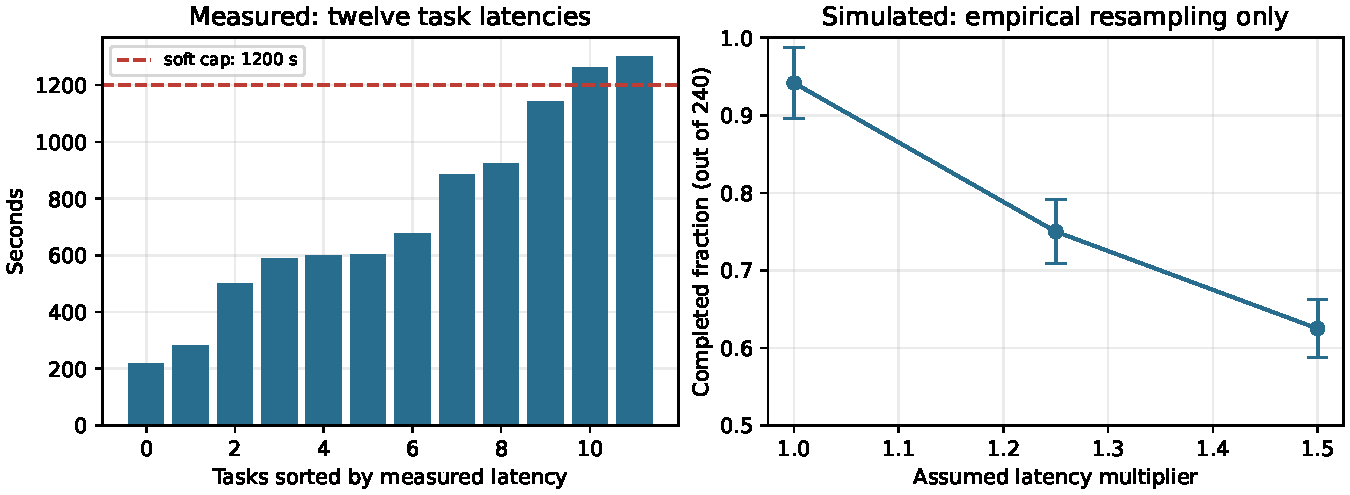
\includegraphics[width=\linewidth]{figures/fig09_audit_sensitivity.pdf}
\caption{Measured latency (left) versus explicitly simulated throughput sensitivity (right). Error bars are the 5th--95th percentiles of empirical resampling; they are not hidden-set confidence intervals. The soft cap can be exceeded.}
\end{figure}

\section{Scores and submission eligibility}
The team's counted main-track entry (31 October 2026) scored 0.00. Submission 57901718 from our \texttt{arc-nvarc-validated} notebook v3 received a public score of 30.56 but was classified late and excluded from the standings. This is a 30.56-point \emph{score difference}, not a threefold increase from zero. The historical leaderboard snapshot lists the team at rank 3599/3627. A score of 30.56 appears near position 1271 in that snapshot, but that is a comparison only, not our official rank.

The reproduction was submitted on 2 November at 08:28 UTC before the 23:59 close and was still pending at 08:44. The retained record establishes late completion but does not independently determine the exact queue duration or prove that capacity saturation caused it. With runtime $T$, queue delay $Q$, and safety margin $M$, a safe submission must satisfy
\[
t_{\mathrm{submit}}+Q+T+M < t_{\mathrm{close}}.
\]
An unknown queue cannot be guaranteed safe by a fixed ``submit by midday'' rule. Earlier submission would improve eligibility slack; it would not by itself improve the solver's accuracy.

\section{Reproducibility, limitations, and next experiments}
The attached audit bundle contains \texttt{audit\_final.py}, original metric JSONs, the measured latency log, the canonical/search source files needed for verification, \texttt{AUDIT\_FINAL.json}, and the generated figure. The JSON records SHA-256 hashes of audited sources. With NumPy and Matplotlib installed, run the script from its preserved competition-directory layout. It needs no model weights, GPU, credentials, or network access. It performs 34,992 transformation assertions, shape-collision and scheduler boundary checks, and metric recounts before writing the simulation outputs.

We do not present a new GPU rerun, an accuracy improvement from canonical repair, or a held-out comparison of alternative schedulers. Twelve durations support only conditional resampling. The metric artifacts are historical and partly version-mismatched. The public LLM may be contaminated, source weights are externally supplied, and no private test labels are available. These limitations exclude claims of state-of-the-art reasoning or a guaranteed top placement.

The next defensible experiments are: (1) measure oracle candidate accuracy separately from selection accuracy on an untouched split; (2) compare original versus repaired canonicalisation with all other search settings fixed; (3) instrument per-scoring-unit prediction availability, fallbacks and success; and (4) evaluate scheduling policies using jointly observed latency and correctness rather than assuming constant $p$. None has been run here. Our final contribution is an executable diagnosis of where apparent progress can be an artefact of metric naming, quotient-state handling, or submission protocol.

\begin{thebibliography}{9}
\bibitem{arcagi2} F. Chollet, M. Knoop, G. Kamradt, B. Landers, and H. Pinkard. \emph{ARC-AGI-2: A New Challenge for Frontier AI Reasoning Systems}. arXiv:2505.11831, 2025 (v2, 2026). \url{https://arxiv.org/abs/2505.11831}
\bibitem{source} Kaggle user \texttt{koushikrudra}. \emph{Failed in AIMO}, notebook version 1, Apache-2.0. \url{https://www.kaggle.com/code/koushikrudra/failed-in-aimo}
\bibitem{model} Kaggle user \texttt{sorokin}. \emph{Qwen3 4B grids15 SFT139}, model version 1. \url{https://www.kaggle.com/models/sorokin/qwen3_4b_grids15_sft139}
\end{thebibliography}
\end{document}
